\documentclass[12pt]{article}

\usepackage{multirow}
\usepackage{tabularx}
\usepackage[table]{xcolor}
\usepackage{textcomp}
\usepackage{booktabs}
\usepackage{ltablex}
\usepackage{graphicx}
\usepackage{float}
\usepackage{capt-of}

\pagestyle{plain}
\setcounter{secnumdepth}{5}

\topmargin=0cm
\oddsidemargin=0cm
\textheight=22.0cm
\textwidth=16cm
\parindent=0cm
\parskip=0.15cm
\topskip=0truecm
\raggedbottom
\abovedisplayskip=3mm
\belowdisplayskip=3mm
\abovedisplayshortskip=0mm
\belowdisplayshortskip=2mm
\normalbaselineskip=12pt
\normalbaselines

\begin{document}

\thispagestyle{empty}
\vspace*{0.5in}
\centerline{\bf\Large Design Document}

\vspace*{0.5in}
\centerline{\bf\Large Team PI-b}

\vspace*{0.5in}
\centerline{\bf\Large 17 March 2019}

\vspace*{1.5in}
\begin{table}[htbp]
\begin{center}
\begin{tabular}{|r | c|}
\hline
Name & ID Number \\
\hline\hline
Simon Huang & 27067380 \\
\hline
Jonathan Massabni & 26337430 \\
\hline
Alexia Soucy & 40014822 \\
\hline
Anthony Funiciello& 40054110\\
\hline
David Gray&40055149\\
\hline
Mair Elbaz&40004558\\
\hline
Rani Rafid&26975852\\
\hline
\end{tabular}
\end{center}
\end{table}

\clearpage
%==============TABLE OF CONTENTS===========
\centerline{\bf\Large TABLE OF CONTENTS}
%\vspace*{0.5in}

\tableofcontents

\newpage
%==============LIST OF FIGURES============
\centerline{\bf\Large LIST OF FIGURES}
%\vspace*{1in}

\listoffigures

\newpage
%===============INTRODUCTION===============

\section{INTRODUCTION}

The purpose of this project is to use software engineering practices to develop a desktop application which plays the Codenames game with NPC's of varying "intelligence." The software was designed using MVC architecture and several common design patterns including the "Strategy Pattern," "Observer Pattern," and "Command Pattern."
\\
\\
This document provides an explanation of our application's architectural and class level software design. The Architectural Design section gives a high level look at how the system is organized using the Model-View-Controller (MVC) architecture. The Detailed Design section describes the design within the subsystems and the purposes of each class. The Dynamic Design Scenarios section explains how the application works by explaining significant execution scenarios of the system.
\\
\\
\newpage
%=================ARCHITECTURAL DESIGN============
\section{ARCHITECTURAL DESIGN}



\subsection{Architectural Diagram}

\begin{figure}[H]
\centering
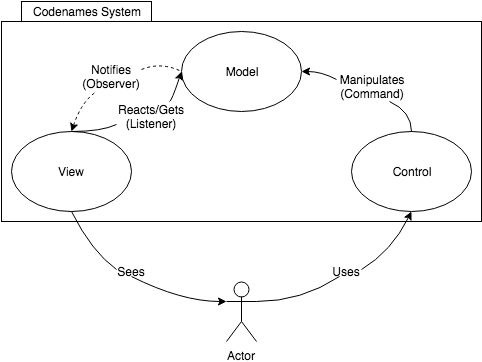
\includegraphics[width=10cm]{Source/MVC.png}
\caption{System Architecture based on Model-View-Control design}
\label{View}
\end{figure}

%A UML class diagram or package diagram depicting the high-level structure of the system,
%accompanied by a one-paragraph text describing the rationale of this design.
%It is mandatory that the system be divided into at least two subsystems,
%and that the purpose of each of these subsystems be exposed here.

%==============

The Codenames game project specifications call for a graphical interface that can reflect an evolving game state and a system through which user input is processed to alter the game state. The application is a layered logical architecture composed of three subsystems inspired and named after the Model-View-Controller (MVC) separation principle. This principle provides a logical approach to dividing the domain, user interface, and application layers into subsystems that can be developed independently and, through interfaces, interact with each other. This section provides a description of the responsibility of each subsystem and discusses the reasoning behind choosing to model this systems architecture according to MVC. \\

The Model subsystem represents the current game state through its three component packages: Board, which represents the data relating to the ongoing game, Player, which represents the players and their strategies (using the Strategy pattern), and Util, which logs everything that takes place in Model. In general, the Model subsystem is synonymous to the domain layer, and is therefore an inspirational creation of the domain model. \\

The View subsystem contains all objects that provide a user-friendly interface to the Codenames game. These objects are responsible for capturing input, and output. They may sometimes produce graphical elements. However, they are not responsible for containing data pertaining to the state of the game, nor do they incorporate any logical behaviour affecting the internals of the application. In the Codenames application, the View subsystem uses the Observer pattern to bind itself to specific Subject classes in the Model subsystem to display the current game state in real time. This allows the Model subsystem to function uninterrupted, independently of the View subsystem. \\

The Control subsystem contains all objects tasked with defining the stimulus and/or handling stimuli forwarded by the View subsystem. In this context, a stimulus is defined as a request, or message that initiates work to be performed by the system. Furthermore, objects in this subsystem possess functional characteristics. In the Codenames application, the game progresses through one turn when the user presses the "Enter" key. The action of a user pressing “Enter” is handled by the GameHandler, which through the Command design pattern, commands the Model classes to do the next turn, changing the Models state, and updating the View accordingly. \\

\subsection{Subsystem Interface Specifications}
In general, the Model and View  according to the Observer design pattern, and the Controller controls the Model by making commands through the Command design pattern. This section specifies the actual function calls which make up these software interfaces between the three (MVC) subsystems. Outside of the two design patterns defined about, most of the Model's interface is functions called by View classes to get the internal state of the game, on which the GUI is based.

\subsubsection {Model Subsystem Interface}
The communication between the Model and View subsystems is implemented in the Observer Design Pattern. As a result, the Model contains classes which extend the Subject abstract class, to which Observer classes in the View may attach() themselves, so that they are notified to changes in the Subject's state. The GameManager, Verbose, and Card classes are Subjects.

\textbf{Subject} An abstract class for Subject's in the Observer design pattern.
\begin{itemize}
  \item void attach(Observer o): add the Observer object o to the list of Observers to be notified upon changes of state.
  \item String getStringProperty(): returns the Subject's state in the form of a String.
  \item CardType getTypeProperty(): returns the Subject's state in the form of a CardType (Red, Blue, Assassin, Bystander).
\end{itemize}

\textbf{GameManager} The GameManager class keeps track of much of the state of the game. It is a Subject, serving as an interface for the View to get data on the games state. Along with the methods of Subject, the GameManager class has the following methods:
\begin{itemize}
  \item void doNextTurn(): The main interface between the Controller and the Model. This initiates the Model to do the next turn, changing the state of the game.
  \item Clue getCurrentClue(): Returns the Clue given by the current team.
  \item int getBlueScore(): Returns the number of cards left for Blue to guess.
  \item int getRedScore(): Returns the number of cards left for Red to guess.
  \item CardType getWinner(): Returns void if nobody has yet won, or CardType.Blue, or CardType.Red if there has been a winner.
\end{itemize}

\textbf{CardBuilder} The CardBuilder class is a helper class for extracting the word data from the .txt files, and turning it into a randomized board. It is used to start a game.
\begin{itemize}
  \item Card[] buildAll(): Returns 25 Cards, generated from the database of nouns and keycards. Used to initialize the game.
\end{itemize}

\textbf{Verbose} The Verbose class is used for logging in the Model. It is a Subject. It uses the Subject's getStringProperty() method to notify its Observers of log messages. It is a Singleton, and as a result has the following methods:
\begin{itemize}
  \item get() Returns the one instance of Verbose.
  \item bind(Observer) attaches Observers to the instance of Verbose.
\end{itemize}

\subsubsection {View Subsystem}
The View subsystem will start by calling start(Stage) that will create a new verboseView and Verbose object.
Codenames class is also responsible for building the GameScene this class calls build(Subject[], Event\textless KeyEvent\textgreater ) of type scene that will set up user input to send to the CardPane class. After GameScene create a CardPane object, it will hold the images of the cards and where each card is place on the board to display. The Verbose object will call bind(Observer) to bind an Observer object to the game board to record events. log(String) will capture events and convert them to phrases that will display in VerboseView. Lastly, a Subject object can call attach(Observer) to attach a new Observer to it which will keep track of things in the Model subsystem.

\textbf{CardPane} A class that implements the Observer to represent the GUI of 1 card on the board. It is covered until the update function is called.
\begin{itemize}
  \item update() Called by subject of class to reveal color of card with image.
\end{itemize}

\subsubsection {Control Subsystem}
The control subsystem creates the command package. Codename's start(Stage) will create a new GameHandler object. This will contain information about the model's GameManager, the View's score and verbose and the control's commandManager and store a history of used commands. The handle(KeyEvent) will control the action on which key is pressed to execute the appropriate command and change the state of the game in the model. After GameHandler, creates a CommandManager, it will be able to create and execute() Command objects. GameHandler also makes a NextTurnCommand object that controls the turn flow of the game to set the input to match the game's commands.\\

The Difficulty class sets the different strategies that each player type will be able to use. Using setDifficulty(), the user is able to select their difficulty and use the appropriate strategy that is stored in the model subsystem. 

\textbf{GameControls} A class responsible for handling the events of restarting or quitting the game. The game board will be reset upon restarting the game or will terminate upon selecting quit.
\begin{itemize}
  \item setEvents() Sets the menu items and actions for the game which includes (Restart) and (Quit).
  \item setAbout() Sets the description of the menu items in a new window.
\end{itemize}



\newpage

%===============MODULE=================
\subsubsection{Package Board}
The Board subsystem of the Model contains the classes which represent the data and state of the Codenames game. This includes classes for game objects such as Card, Board, KeyCard, Clue, and CardType. The subsystem also contains classes which are used to initialize these game objects. The GameManager class includes references to the game objects being played with, and the Players playing the game. The GameManager also contains methods which modify the game state by making players take turns. The Controller's Commands to the Model contain function calls to the GameManager class.

\paragraph{Detailed Design Diagram}\mbox{}
\begin{figure}[H]
\centering
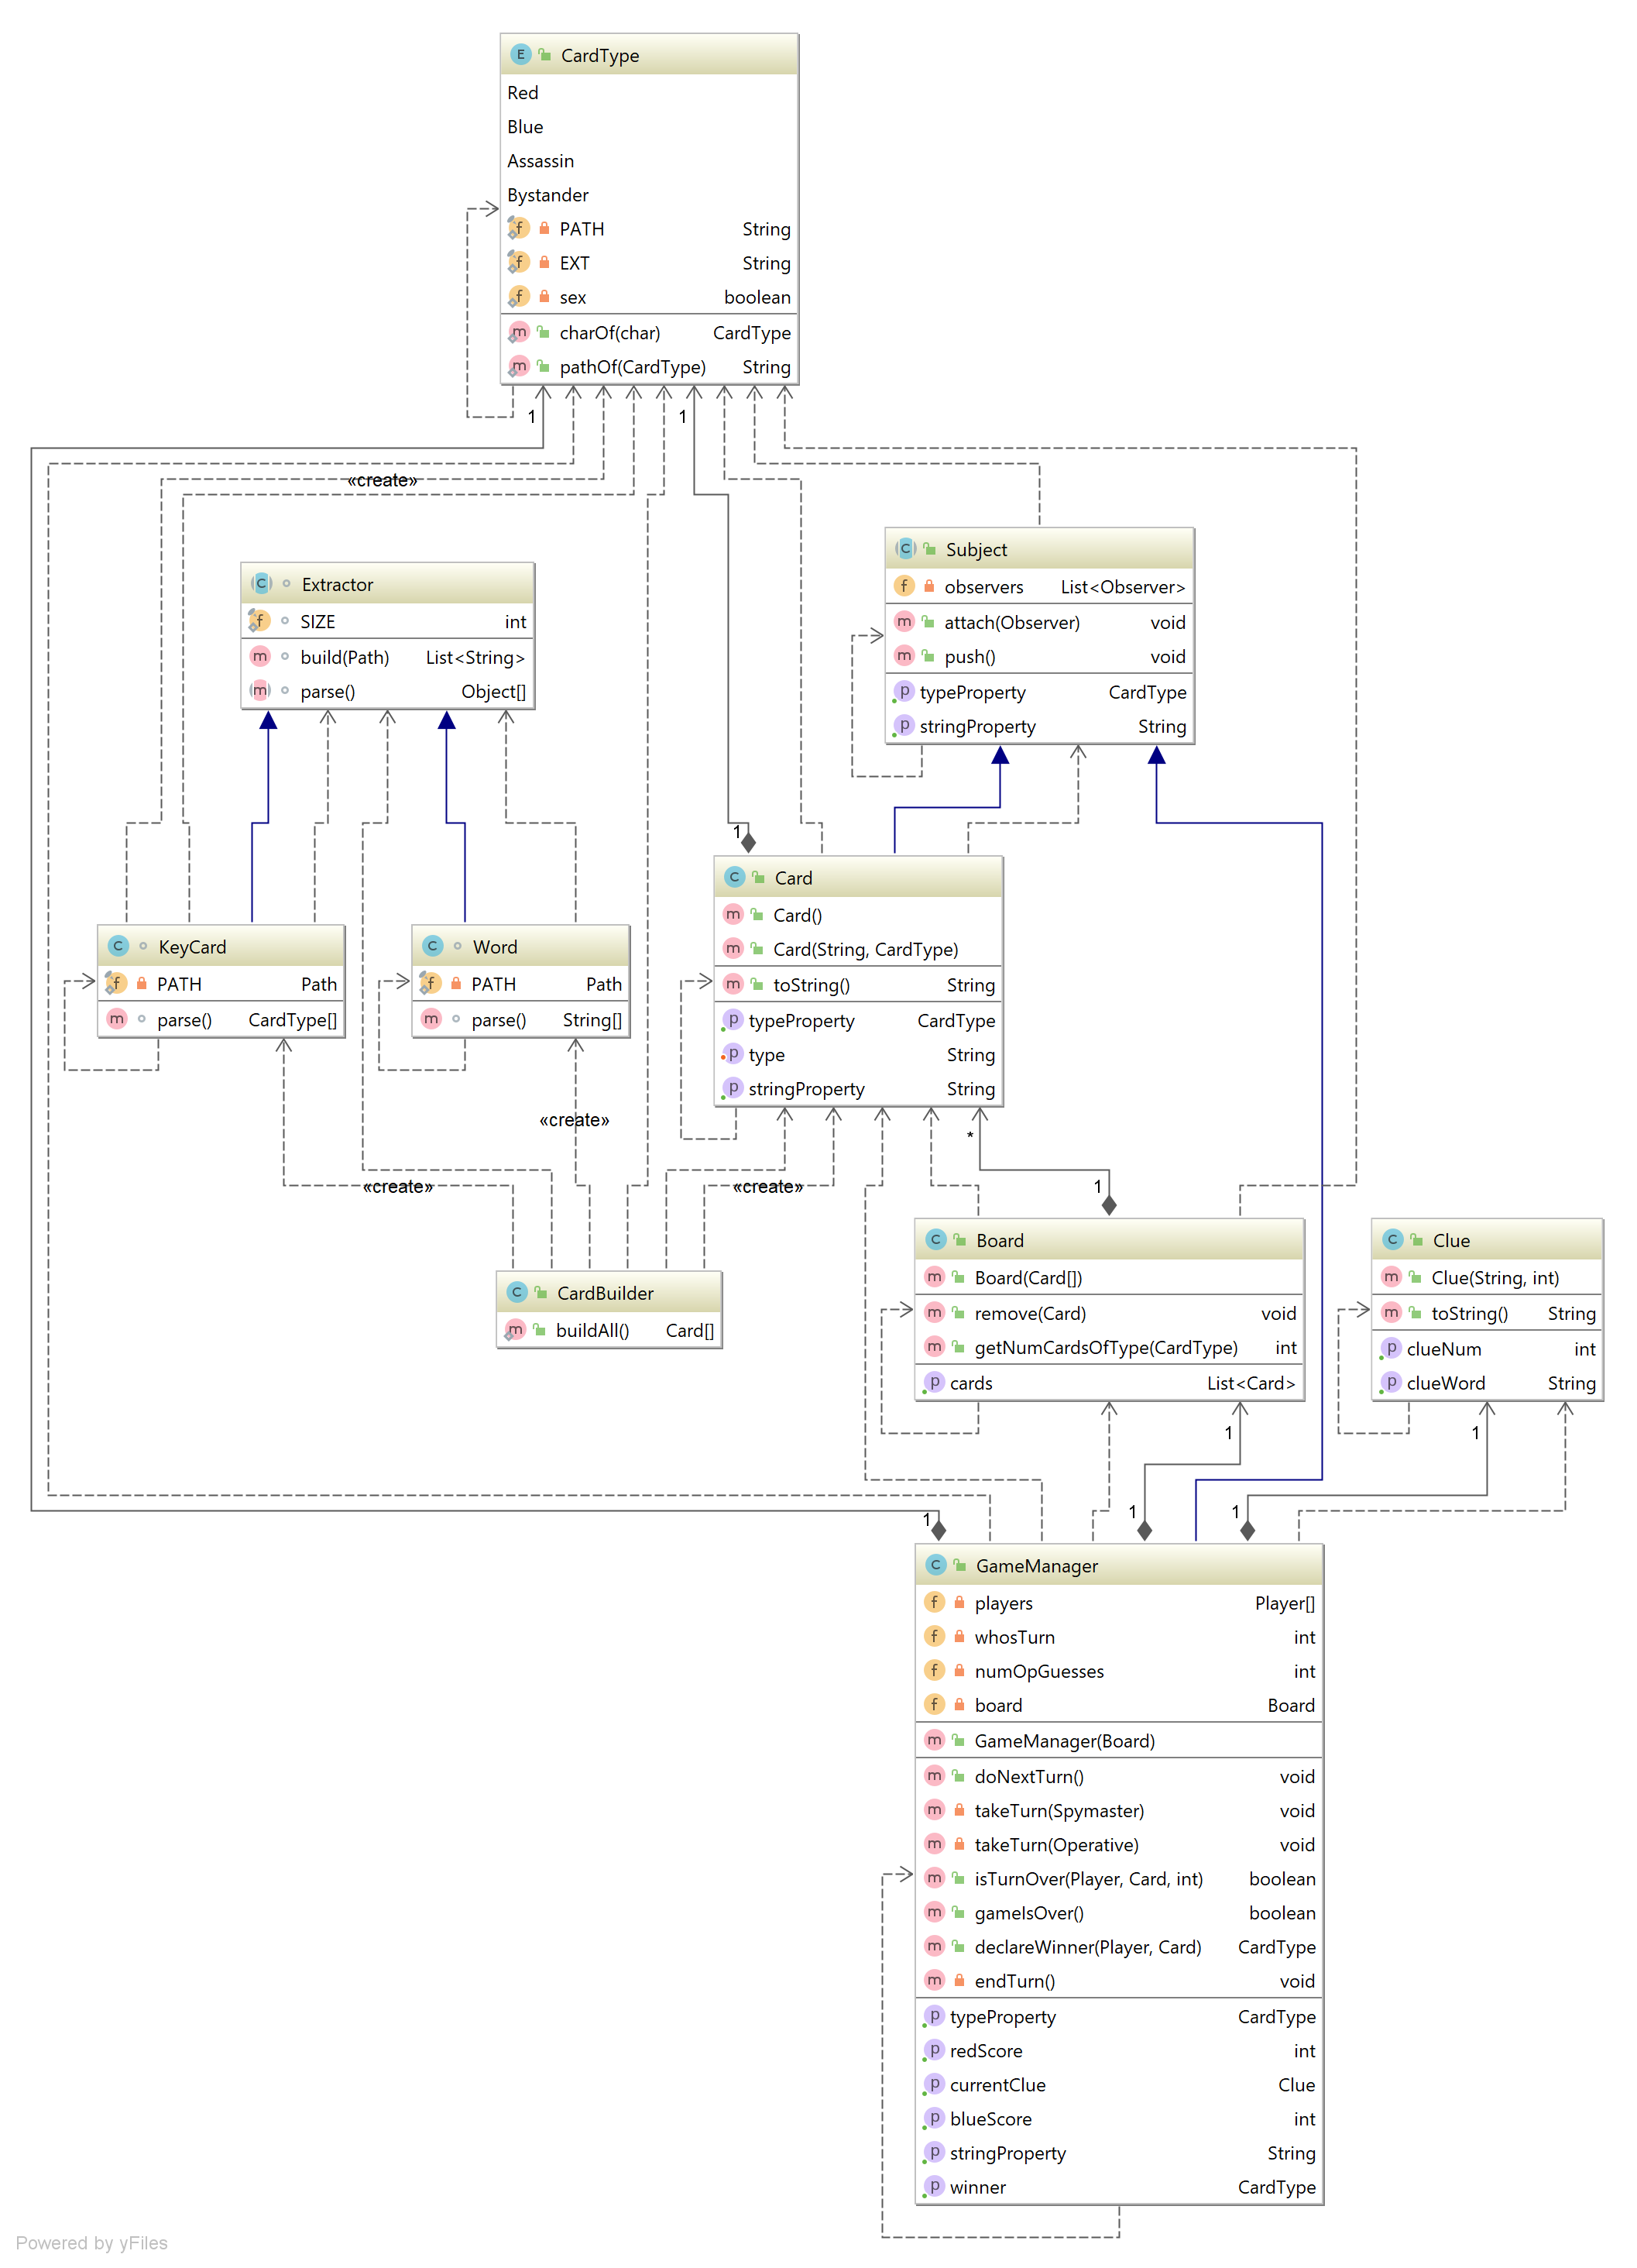
\includegraphics[width=8cm]{Source/Module/Model/Board/Model_Board.png}
\caption{UML Diagram of Package Board in Module Model}
\end{figure}

\paragraph{Class Bipartite}\mbox{}
\begin{tabularx}{\textwidth}{|c||l|p{2.75cm}|l|X|}
    \hline
    \cellcolor{lightgray}Class Name & \multicolumn{4}{X|}{Bipartite}\\
    \hline
    \cellcolor{lightgray}Inherits From & \multicolumn{4}{X|}{None}\\
    \hline
    \cellcolor{lightgray}Description & \multicolumn{4}{p{12cm}|}{Creates a bipartite graph showing the relation between words and clues.}\\
    \hline\hline
    
    \cellcolor{lightgray}Attributes & \cellcolor{lightgray}Visibility & \cellcolor{lightgray}Data type & \cellcolor{lightgray}Name & \cellcolor{lightgray}Description\\\cline{2-5}
    \cellcolor{lightgray} & Private & HashMultiMap \textlangle{}String, String\textrangle{} & wordsToClues & The map from words to clues.\\
    \hline
    \cellcolor{lightgray} & Private & HashMultiMap \textlangle{}String, String\textrangle{} & cluesToWords & The map from clues to words. (One clue can be associated with multiple words)\\
    \hline\hline
    
    \cellcolor{lightgray}Methods & \cellcolor{lightgray}Visibility & \multicolumn{2}{l|}{\cellcolor{lightgray}Method Name} & \cellcolor{lightgray}Description\\\cline{2-5}
    \cellcolor{lightgray} & Public & \multicolumn{2}{l|}{Bipartite(Board board)} & Constructor; creates empty hashMultiMaps and sets them to the board's variables, then processes them.\\
    \hline
    \cellcolor{lightgray} & Private & \multicolumn{2}{l|}{processCards(Board board)} & Creates a bipartite graph with only the words on the current board.\\
    \hline
    \cellcolor{lightgray} & Public & \multicolumn{2}{l|}{getWordsToClues()} & Returns the hash map that contains the mapping of words to clues.\\
    \hline
    \cellcolor{lightgray} & Public & \multicolumn{2}{l|}{getCluesToWords()} & Returns the hash map that contains the mapping of clues to words.\\
    \hline
    \cellcolor{lightgray} & Public & \multicolumn{2}{l|}{getClue(String cardWord)} & Returns a string representation of a clue.\\
    \hline
    \cellcolor{lightgray} & Public & \multicolumn{2}{l|}{removeWord(String word)} & Removes a word from the bipartite including its related clues.\\
    \hline
    \cellcolor{lightgray} & Private & \multicolumn{2}{l|}{debug()} & Prints the current status of the bipartite.\\
    \hline
    
\end{tabularx}
\paragraph{Class Board}\mbox{}
 \begin{tabularx}{\textwidth}{|c||l|l|l|X|}
    \hline
    \cellcolor{lightgray}Class Name & \multicolumn{4}{X|}{Board}\\
    \hline
    \cellcolor{lightgray}Inherits From & \multicolumn{4}{X|}{None}\\
    \hline
    \cellcolor{lightgray}Description & \multicolumn{4}{p{12cm}|}{The board stores the set of code name Cards on the board, which have not yet been guessed.}\\
    \hline\hline
    \cellcolor{lightgray}Attributes & \cellcolor{lightgray}Visibility & \cellcolor{lightgray}Data type & \cellcolor{lightgray}Name & \cellcolor{lightgray}Description\\\cline{2-5}
    \cellcolor{lightgray} & Private & List of Cards & cards & Holds the set of Cards that have not yet been guessed by Operatives\\
    \hline\hline
    
    \cellcolor{lightgray}Methods & \cellcolor{lightgray}Visibility & \multicolumn{2}{l|}{\cellcolor{lightgray}Method Name} & \cellcolor{lightgray}Description\\\cline{2-5}
    \cellcolor{lightgray} & Public & \multicolumn{2}{l|}{Board(Card[] cards)} & Initializes the board with a list of cards.\\
    \hline
    \cellcolor{lightgray} & Public & \multicolumn{2}{l|}{remove(Card c)} & Remove the specified card from the set of unchosen cards.\\
    \hline
    \cellcolor{lightgray} & Public & \multicolumn{2}{l|}{getCards()} & Return all of the unchosen cards still available, as a List.\\
    \hline
    \cellcolor{lightgray} & Public & \multicolumn{2}{X|}{getNumCardsOfType (CardType type)} & Return integer count of the number of unchosen cards left with color specified by variable type.\\
    \hline
\end{tabularx}
\paragraph{Class Card}\mbox{}
\begin{tabularx}{\textwidth}{|c||l|l|l|X|}
    \hline
    \cellcolor{lightgray}Class Name & \multicolumn{4}{X|}{Card}\\
    \hline
    \cellcolor{lightgray}Inherits From & \multicolumn{4}{X|}{Extends Subject}\\
    \hline
    \cellcolor{lightgray}Description & \multicolumn{4}{p{12cm}|}{The Card class represents a single codenames card, and it's true identity (color). It is a subject in the observer pattern, because the view's CardPanes each individually observe a card.}\\
    \hline\hline
    \cellcolor{lightgray}Attributes & \cellcolor{lightgray}Visibility & \cellcolor{lightgray}Data type & \cellcolor{lightgray}Name & \cellcolor{lightgray}Description\\\cline{2-5}
    \cellcolor{lightgray} & Private & String & word & The codename word.\\
    \hline
    \cellcolor{lightgray} & Private & CardType & type & The true identity of the card: Blue, Red, Assassin, or Bystander.\\
    \hline\hline
    \cellcolor{lightgray}Methods & \cellcolor{lightgray}Visibility & \multicolumn{2}{l|}{\cellcolor{lightgray}Method Name} & \cellcolor{lightgray}Description\\\cline{2-5}
    \cellcolor{lightgray} & Public & \multicolumn{2}{l|}{Card()} & Default constructor; initializes word and type to null.\\
    \hline
    \cellcolor{lightgray} & Public & \multicolumn{2}{X|}{Card (String word, CardType type)} & Constructor.\\
    \hline
    \cellcolor{lightgray} & Public & \multicolumn{2}{l|}{setType(String word)} & Sets the codename on this card. \\
    \hline
    \cellcolor{lightgray} & Public & \multicolumn{2}{l|}{toString()} & Returns the codename. Could be changed to return color and word. \\
    \hline
    \cellcolor{lightgray} & Public & \multicolumn{2}{l|}{getStringProperty()} & Returns the codename. This overrides a method of Subject. \\
    \hline
    \cellcolor{lightgray} & Public & \multicolumn{2}{l|}{getTypeProperty()} & Returns the cards true identity (color). This overrides a method of Subject. \\
    \hline
\end{tabularx}
\paragraph{Class Extractor}\mbox{}
\begin{tabularx}{\textwidth}{|c||l|l|l|X|}
    \hline
    \cellcolor{lightgray}Class Name & \multicolumn{4}{X|}{Extractor}\\
    \hline
    \cellcolor{lightgray}Inherits From & \multicolumn{4}{X|}{None}\\
    \hline
    \cellcolor{lightgray}Description & \multicolumn{4}{p{12cm}|}{Abstract class extractor abstracts the process of ingesting 25 random lines of a file. This process is done in creating the KeyCard from the database of keycards, and for choosing 25 codenames.}\\
    \hline\hline
    \cellcolor{lightgray}Attributes & \cellcolor{lightgray}Visibility & \cellcolor{lightgray}Data type & \cellcolor{lightgray}Name & \cellcolor{lightgray}Description\\\cline{2-5}
    \cellcolor{lightgray} & Private & final int & SIZE & The number of cards in a board. 25.\\
    \hline\hline
    \cellcolor{lightgray}Methods & \cellcolor{lightgray}Visibility & \multicolumn{2}{l|}{\cellcolor{lightgray}Method Name} & \cellcolor{lightgray}Description\\\cline{2-5}
    \cellcolor{lightgray} & Public & \multicolumn{2}{l|}{build(Path path)} & Returns every line of the file at Path path as a list.\\
    \hline
    \cellcolor{lightgray} & abstract & \multicolumn{2}{l|}{parse()} & To be overridden by any Extractor, to return a list of whatever objects the class is creating from the data it extracts.\\
    \hline
\end{tabularx}
\paragraph{Class Word}\mbox{}
\begin{tabularx}{\textwidth}{|c||l|l|l|X|}
    \hline
    \cellcolor{lightgray}Class Name & \multicolumn{4}{X|}{Word}\\
    \hline
    \cellcolor{lightgray}Inherits From & \multicolumn{4}{X|}{extends Extractor}\\
    \hline
    \cellcolor{lightgray}Description & \multicolumn{4}{p{12cm}|}{Extracts words from a file and returns the first 25.}\\
    \hline\hline
    \cellcolor{lightgray}Attributes & \cellcolor{lightgray}Visibility & \cellcolor{lightgray}Data type & \cellcolor{lightgray}Name & \cellcolor{lightgray}Description\\\cline{2-5}
    \cellcolor{lightgray} & Private & final Path & PATH & The path to the .txt file containing the codenames.\\
    \hline\hline
    \cellcolor{lightgray}Methods & \cellcolor{lightgray}Visibility & \multicolumn{2}{l|}{\cellcolor{lightgray}Method Name} & \cellcolor{lightgray}Description\\\cline{2-5}
    \hline
    \cellcolor{lightgray} & Public & \multicolumn{2}{l|}{parse()} & Calls build() and returns only the first 25 elements of the randomly ordered list of Strings (to be codenames).\\
    \hline
\end{tabularx}
\paragraph{Class KeyCard}\mbox{}

\begin{tabularx}{\textwidth}{|c||l|l|l|X|}
    \hline
    \cellcolor{lightgray}Class Name & \multicolumn{4}{X|}{KeyCard}\\
    \hline
    \cellcolor{lightgray}Inherits From & \multicolumn{4}{X|}{extends Extractor}\\
    \hline
    \cellcolor{lightgray}Description & \multicolumn{4}{p{12cm}|}{Extracts all of the data representing KeyCards from a text file, then chooses a random one and parses it into a List of CardTypes.}\\
    \hline\hline
    
    \cellcolor{lightgray}Methods & \cellcolor{lightgray}Visibility & \multicolumn{2}{l|}{\cellcolor{lightgray}Method Name} & \cellcolor{lightgray}Description\\\cline{2-5}
    \hline
    \cellcolor{lightgray} & Public & \multicolumn{2}{l|}{parse()} & Uses build() to get the possible Key Cards in a random order, then takes the first one and maps each character to a CardType to create a list of CardTypes.\\
    \hline
\end{tabularx}
\paragraph{Class CardBuilder}\mbox{}
\begin{tabularx}{\textwidth}{|c||l|l|l|X|}
    \hline
    \cellcolor{lightgray}Class Name & \multicolumn{4}{X|}{CardBuilder}\\
    \hline
    \cellcolor{lightgray}Inherits From & \multicolumn{4}{X|}{None}\\
    \hline
    \cellcolor{lightgray}Description & \multicolumn{4}{p{12cm}|}{Creates an array of Card objects based on a random selection of 25 words and a key card.}\\
    \hline\hline
    
    \cellcolor{lightgray}Methods & \cellcolor{lightgray}Visibility & \multicolumn{2}{l|}{\cellcolor{lightgray}Method Name} & \cellcolor{lightgray}Description\\\cline{2-5}
    \cellcolor{lightgray} & Public & \multicolumn{2}{l|}{buildAll()} & Use the KeyCard and Word classes to create an array of 25 Cards (the core of the board).\\
    \hline
    
\end{tabularx}
\paragraph{Class CardType}\mbox{}
\begin{tabularx}{\textwidth}{|c||l|l|l|X|}
    \hline
    \cellcolor{lightgray}Class Name & \multicolumn{4}{X|}{CardType}\\
    \hline
    \cellcolor{lightgray}Inherits From & \multicolumn{4}{X|}{None}\\
    \hline
    \cellcolor{lightgray}Description & \multicolumn{4}{p{12cm}|}{An enum type which represents the possible colours of a card on a Key Card. Blue, Red, Assassin, or Bystander. Can also be used for team colour.}\\

    \hline\hline
    \cellcolor{lightgray}Attributes & \cellcolor{lightgray}Visibility & \cellcolor{lightgray}Data type & \cellcolor{lightgray}Name & \cellcolor{lightgray}Description\\\cline{2-5}
    \cellcolor{lightgray} & Private & String & PATH & The path to the images used by the GUI to represent the colours on the board.\\
    \hline    
    \cellcolor{lightgray} & Private & String & EXT & The file extension of the images used by the GUI to represent the colours on the board.\\
    \hline    
    \cellcolor{lightgray} & Private & boolean & sex & For the GUI, some cards should be displayed as male spys and some should be female.\\
    \hline\hline
    \cellcolor{lightgray}Methods & \cellcolor{lightgray}Visibility & \multicolumn{2}{l|}{\cellcolor{lightgray}Method Name} & \cellcolor{lightgray}Description\\\cline{2-5}
    \hline
    \cellcolor{lightgray} & Public & \multicolumn{2}{l|}{charOf(char arg)} & Each CardType is represented in the database as a character in a String. charOf returns the CardType represented by a character. B is Blue, R is Red, Y is Bystander, A is Assassin.\\
    \hline
    \cellcolor{lightgray} & Public & \multicolumn{2}{l|}{pathOf(CardType type)} & Returns the path to the image which can be used to display this colour on the board GUI.\\
    \hline
\end{tabularx}
\paragraph{Class Clue}\mbox{}

\begin{tabularx}{\textwidth}{|c||l|l|l|X|}
    \hline
    \cellcolor{lightgray}Class Name & \multicolumn{4}{X|}{Clue}\\
    \hline
    \cellcolor{lightgray}Inherits From & \multicolumn{4}{X|}{None}\\
    \hline
    \cellcolor{lightgray}Description & \multicolumn{4}{p{12cm}|}{Represents a Clue given by a SpyMaster. Keeps track of the clue word and the number of associated cards. }\\

    \hline\hline
    \cellcolor{lightgray}Attributes & \cellcolor{lightgray}Visibility & \cellcolor{lightgray}Data type & \cellcolor{lightgray}Name & \cellcolor{lightgray}Description\\\cline{2-5}
    \cellcolor{lightgray} & Private & String & clueWord & The word part of the clue.\\
    \hline    
    \cellcolor{lightgray} & Private & int & clueNum & The number part of the clue. Should represent the number of Cards associated with the word. \\
    \hline\hline
    \cellcolor{lightgray}Methods & \cellcolor{lightgray}Visibility & \multicolumn{2}{l|}{\cellcolor{lightgray}Method Name} & \cellcolor{lightgray}Description\\\cline{2-5}
    \hline
    \cellcolor{lightgray} & Public & \multicolumn{2}{X|}{Clue(String clueWord, int clueNum)} & Constructor.\\
    \hline
    \cellcolor{lightgray} & Public & \multicolumn{2}{l|}{getClueWord()} & Getter for the clue word. \\
    \hline
    \cellcolor{lightgray} & Public & \multicolumn{2}{l|}{getClueNum()} & Getter for the clue number. \\
    \hline
    \cellcolor{lightgray} & Public & \multicolumn{2}{l|}{toString()} & Clue represented as a string. Could be "Word:Num".\\
    \hline
\end{tabularx}
\paragraph{Class Constants}\mbox{}
\begin{tabularx}{\textwidth}{|c||l|l|l|X|}
    \hline
    \cellcolor{lightgray}Class Name & \multicolumn{4}{X|}{Constants}\\
    \hline
    \cellcolor{lightgray}Inherits From & \multicolumn{4}{X|}{None}\\
    \hline
    \cellcolor{lightgray}Description & \multicolumn{4}{p{12cm}|}{Stores any constants used across classes}\\
    \hline\hline
    \cellcolor{lightgray}Attributes & \cellcolor{lightgray}Visibility & \cellcolor{lightgray}Data type & \cellcolor{lightgray}Name & \cellcolor{lightgray}Description\\\cline{2-5}
    \cellcolor{lightgray} & Public & Path & WORDS\textunderscore{}PATH & Path to the words file; used for debug.\\
    \hline    
    \cellcolor{lightgray} & Public & boolean & DEBUG & Debug mode. True.\\
    \hline
\end{tabularx}
\paragraph{Class Subject}\mbox{}
\begin{tabularx}{\textwidth}{|c||l|l|l|X|}
    \hline
    \cellcolor{lightgray}Class Name & \multicolumn{4}{X|}{Subject}\\
    \hline
    \cellcolor{lightgray}Inherits From & \multicolumn{4}{X|}{None}\\
    \hline
    \cellcolor{lightgray}Description & \multicolumn{4}{p{12cm}|}{Part of the Observer pattern. Classes which are to be observable (the subjects) extend this class.}\\
    \hline\hline
    
    \cellcolor{lightgray}Attributes & \cellcolor{lightgray}Visibility & \cellcolor{lightgray}Data type & \cellcolor{lightgray}Name & \cellcolor{lightgray}Description\\\cline{2-5}
    \cellcolor{lightgray} & Private & List of Observers & observers & The set of Observers observing this subject.\\ 
    \hline\hline
    
    \cellcolor{lightgray}Methods & \cellcolor{lightgray}Visibility & \multicolumn{2}{l|}{\cellcolor{lightgray}Method Name} & \cellcolor{lightgray}Description\\\cline{2-5}
    \hline
    \cellcolor{lightgray} & Public & \multicolumn{2}{l|}{attach(Observer observer)} & Adds observer to this Subject's list of observers.\\
    \hline
    \cellcolor{lightgray} & Public & \multicolumn{2}{l|}{push()} & Notify all observerrs that the state of this Subject has changed. \\
    \hline
    \cellcolor{lightgray} & Public & \multicolumn{2}{l|}{getStringProperty()} & Abstract method to be overridden by all Subjects. This is a way for Observers to get state information from the Subject, as a String. \\
    \hline
    \cellcolor{lightgray} & Public & \multicolumn{2}{l|}{getTypeProperty()} & Abstract method to be overridden by all Subjects. This is a way for Observers to get state information from the Subject in the form of a CardType (a color).\\
    \hline
\end{tabularx}
\paragraph{Class GameManager}\mbox{}
\begin{tabularx}{\textwidth}{|c||l|l|l|X|}
    \hline
    \cellcolor{lightgray}Class Name & \multicolumn{4}{X|}{GameManager}\\
    \hline
    \cellcolor{lightgray}Inherits From & \multicolumn{4}{X|}{None}\\
    \hline
    \cellcolor{lightgray}Description & \multicolumn{4}{p{12cm}|}{Keeps track of the games state, including the players, current turn, and current clue. Allows manipulation of game state by initiating the next turn. }\\

    \hline\hline
    \cellcolor{lightgray}Attributes & \cellcolor{lightgray}Visibility & \cellcolor{lightgray}Data type & \cellcolor{lightgray}Name & \cellcolor{lightgray}Description\\\cline{2-5}
    \cellcolor{lightgray} & Private & Player[] & players & Array of players participating in the game. Should be 4 players, in order of when they will take their turn. So Red Spy, Red Op, Blue Spy, Blue Op.\\ 
    \hline
    \cellcolor{lightgray} & Private & int & whosTurn & Index into players to keep track of whos turn it currently is.\\ 
    \hline
    \cellcolor{lightgray} & Private & CardType & winningTeam & Holds the colour of the winning team. Not set if nobody has won yet.\\ 
    \hline
    \cellcolor{lightgray} & Private & Clue & currentClue & Reference to the clue given by the team who is currently taking their turn. \\ 
    \hline
    \cellcolor{lightgray} & Private & int & numOpGuesses & Keeps track of how many guesses the operative has made so far in their turn, as the game must enforce a limit.\\ 
    \hline
    \cellcolor{lightgray} & Private & Board & board & Reference to the Board object the game is being played on. \\ 
    \hline
    \cellcolor{lightgray} & Private & Bipartite & bipartite & Shows the relationship between words and clues. \\ 
    \hline\hline
    
    \cellcolor{lightgray}Methods & \cellcolor{lightgray}Visibility & \multicolumn{2}{l|}{\cellcolor{lightgray}Method Name} & \cellcolor{lightgray}Description\\\cline{2-5}
    \hline
    \cellcolor{lightgray} & Public & \multicolumn{2}{l|}{GameManager(Board board)} & Constructor. Start a game with the board.\\
    \hline
    \cellcolor{lightgray} & Public & \multicolumn{2}{l|}{doNextTurn()} & Make the game run the next turn, changing the state of the game.\\
    \hline
    \cellcolor{lightgray} & Private & \multicolumn{2}{l|}{
    takeTurn(Spymaster p)} & Used by doNextTurn(), if the current player is a Spymaster. Makes the Spymaster take its turn. \\
    \hline
    \cellcolor{lightgray} & Private & \multicolumn{2}{l|}{
    takeTurn(Operative p)} & Used by doNextTurn(), if the current player is an Operative. Makes the Operative take its turn. \\
    \hline
    \cellcolor{lightgray} & Public & \multicolumn{2}{X|}{isTurnOver(Player p, Card guess, int clueNum)} & Tells whether or not the current turn should end based on current state information given. \\
    \hline
    \cellcolor{lightgray} & Public & \multicolumn{2}{X|}{gameIsOver()} & Returns true if a winning team has been determined. \\
    \hline
    \cellcolor{lightgray} & Public & \multicolumn{2}{X|}{declareWinner(Player lastPlayer, Card lastGuess)} & Determines the winner based on the last player's team and what card they last guessed. \\
    \hline
    \cellcolor{lightgray} & Public & \multicolumn{2}{X|}{endTurn()} & Ends the turn and resets the number of guesses. \\
    \hline
    \cellcolor{lightgray} & Public & \multicolumn{2}{X|}{getBlueScore()} & Returns the blue team's current score. \\
    \hline
    \cellcolor{lightgray} & Public & \multicolumn{2}{X|}{getRedScore()} & Returns the red team's current score. \\
    \hline
    \cellcolor{lightgray} & Public & \multicolumn{2}{X|}{getWinner()} & Returns the winning team. \\
    \hline
    \cellcolor{lightgray} & Public & \multicolumn{2}{X|}{getCurrentClue()} & Returns the current given clue. \\
    \hline
    \cellcolor{lightgray} & Public & \multicolumn{2}{X|}{getStringProperty()} & Returns either the current clue or a game over message, depending on current game state. \\
    \hline
    \cellcolor{lightgray} & Public & \multicolumn{2}{X|}{getTypeProperty()} & Returns either the team whose turn it is, or the winning team, depending on game state. \\
    \hline
\end{tabularx}
\paragraph{Class JSONProcessor}\mbox{}
\begin{tabularx}{\textwidth}{|c||l|l|l|X|}
    \hline
    \cellcolor{lightgray}Class Name & \multicolumn{4}{X|}{JSONProcessor}\\
    \hline
    \cellcolor{lightgray}Inherits From & \multicolumn{4}{X|}{None}\\
    \hline
    \cellcolor{lightgray}Description & \multicolumn{4}{p{12cm}|}{Processes a .json file and return a JSON object. Using Simple JSON library}\\
    \hline\hline
    
    \cellcolor{lightgray}Methods & \cellcolor{lightgray}Visibility & \multicolumn{2}{l|}{\cellcolor{lightgray}Method Name} & \cellcolor{lightgray}Description\\\cline{2-5}
    \hline
    \cellcolor{lightgray} & Public & \multicolumn{2}{l|}{ProcessCurrentJSON()} & Processes the current .json file defined in Constants.\\
    \hline
    \cellcolor{lightgray} & Public & \multicolumn{2}{l|}{ProcessCustomJSON(Path path)} & Process any kind of .json file\\
    \hline
    \cellcolor{lightgray} & Public & \multicolumn{2}{l|}{ProcessJSON(Path path)} & Process .json object. If the specified file does not exist, the program will terminate and display the error\\
    \hline
\end{tabularx}
%==================DYNAMIC DESIGN SCENARIOS=================
\subsubsection{Package Board}
The Board subsystem of the Model contains the classes which represent the data and state of the Codenames game. This includes classes for game objects such as Card, Board, KeyCard, Clue, and CardType. The subsystem also contains classes which are used to initialize these game objects. The GameManager class includes references to the game objects being played with, and the Players playing the game. The GameManager also contains methods which modify the game state by making players take turns. The Controller's Commands to the Model contain function calls to the GameManager class.

\paragraph{Detailed Design Diagram}\mbox{}
\begin{figure}[H]
\centering
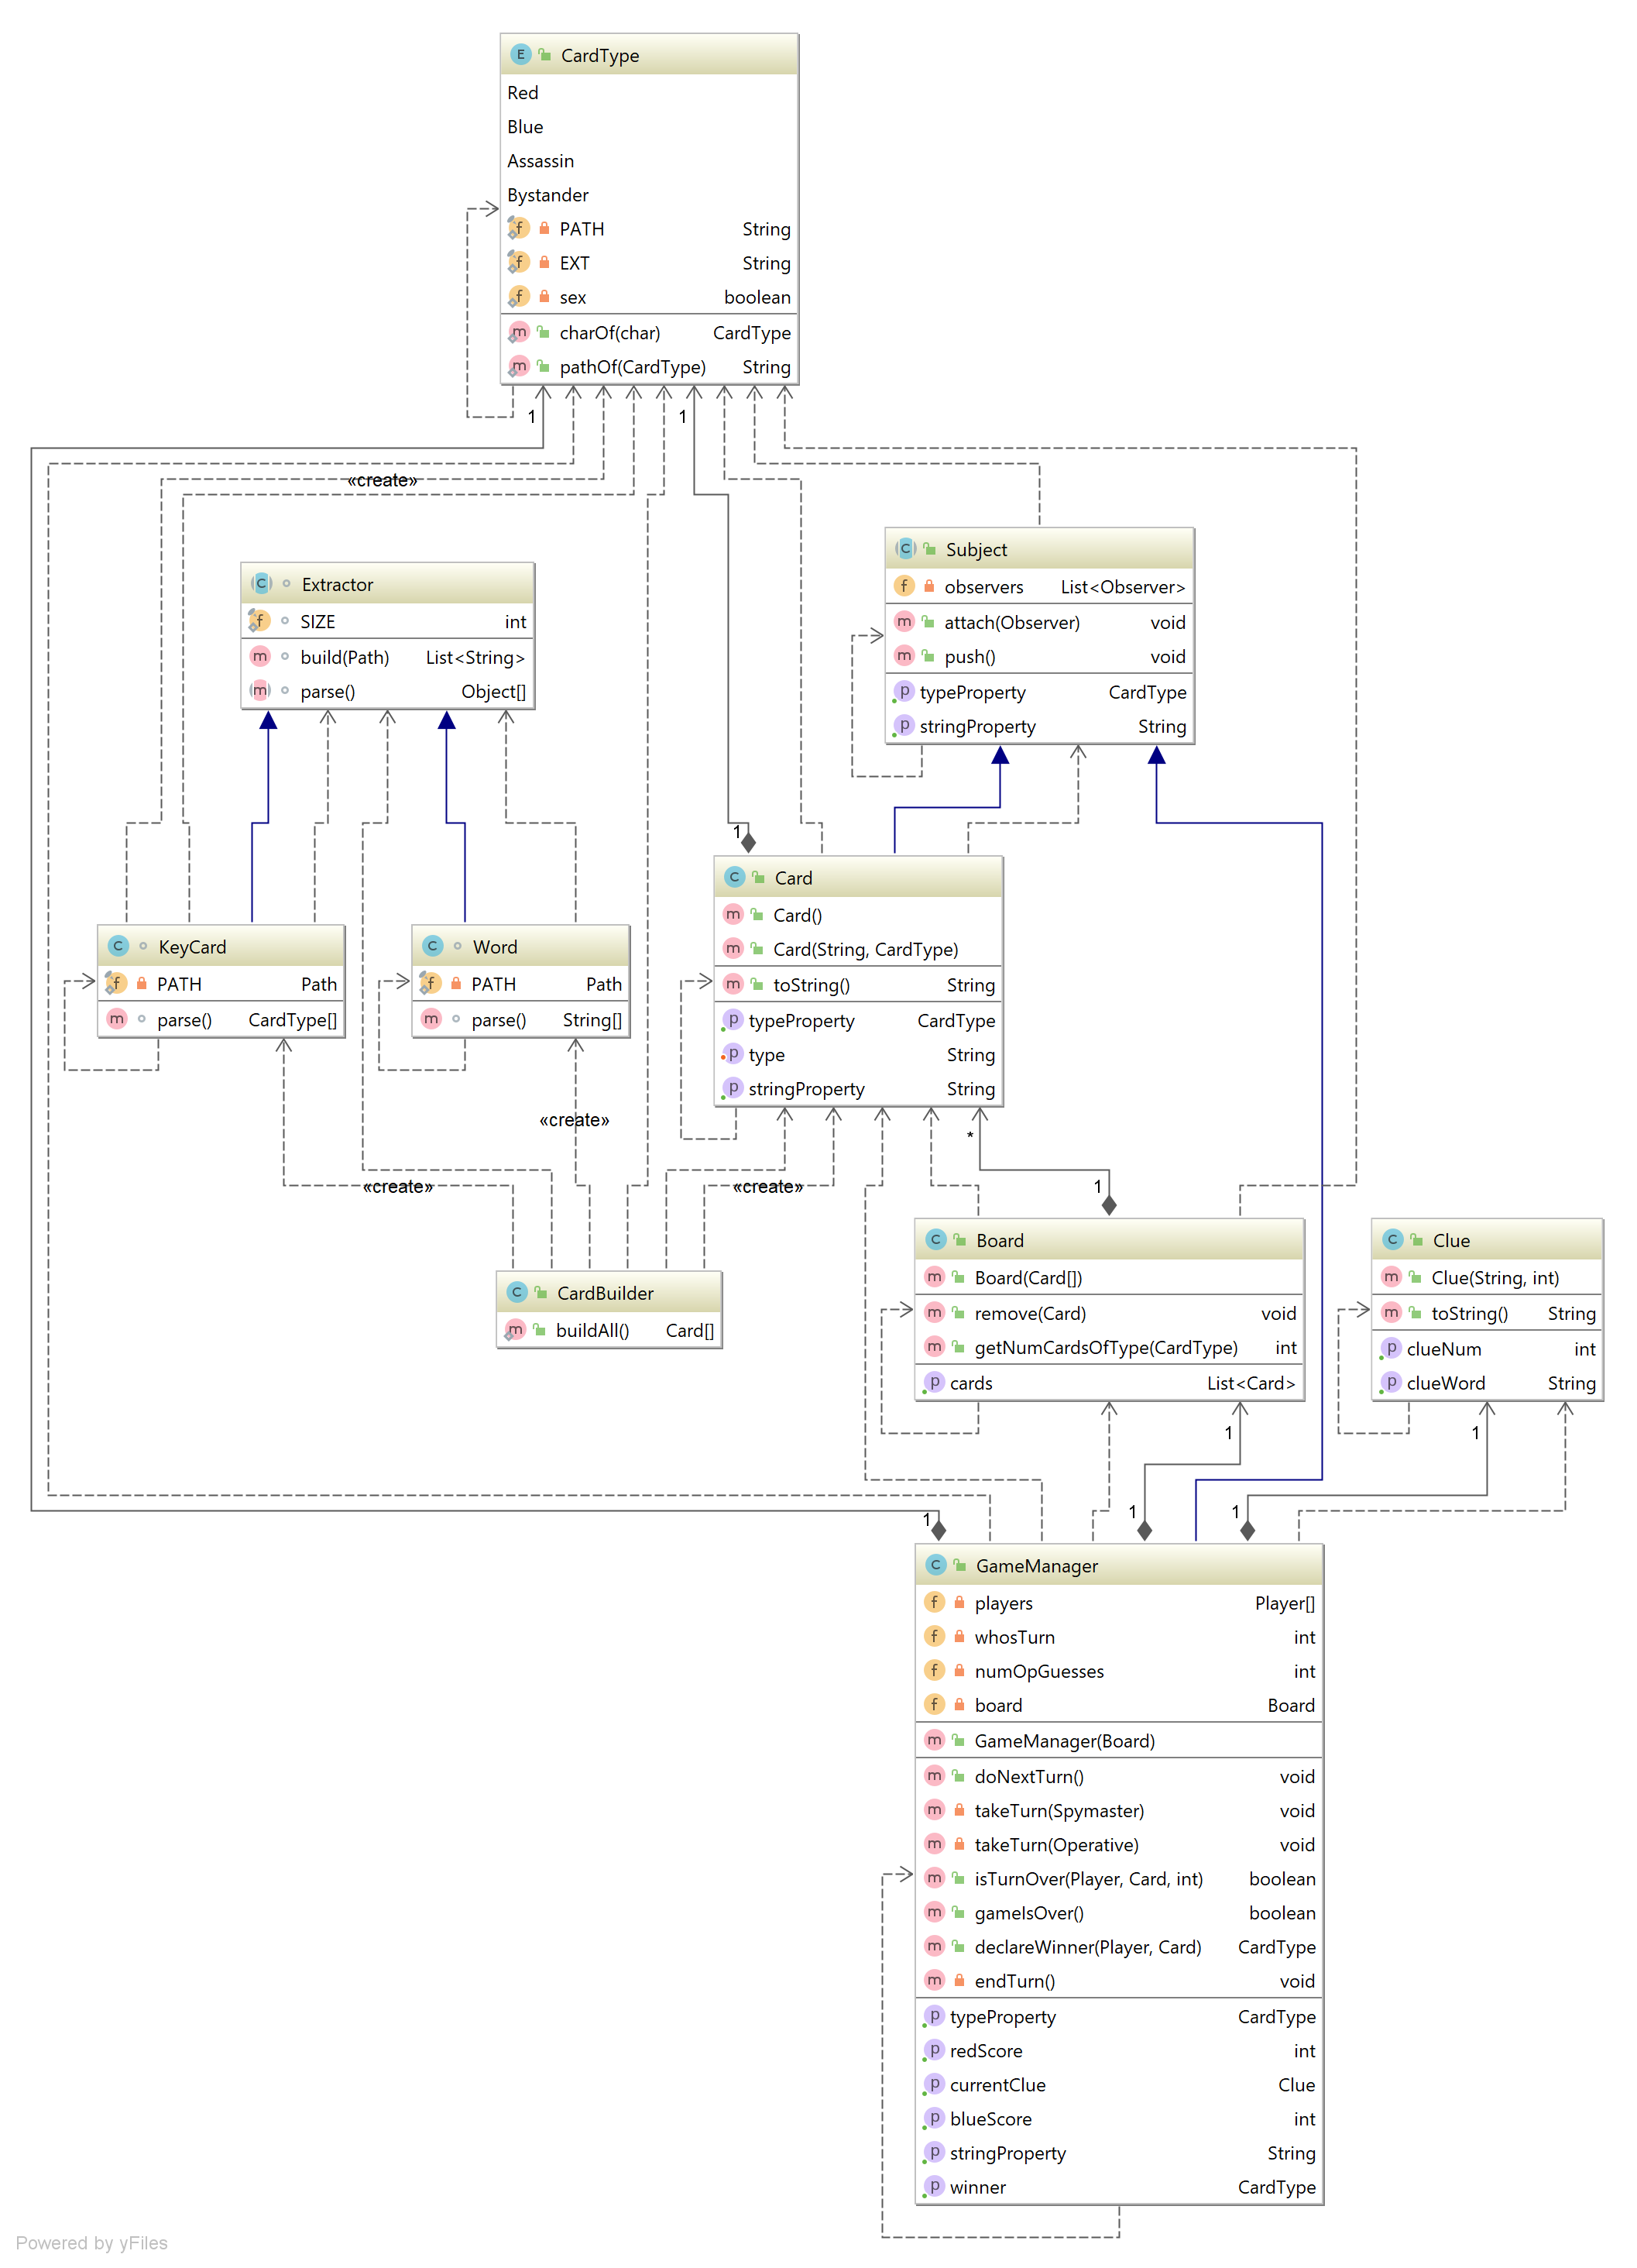
\includegraphics[width=8cm]{Source/Module/Model/Board/Model_Board.png}
\caption{UML Diagram of Package Board in Module Model}
\end{figure}

\paragraph{Class Bipartite}\mbox{}
\begin{tabularx}{\textwidth}{|c||l|p{2.75cm}|l|X|}
    \hline
    \cellcolor{lightgray}Class Name & \multicolumn{4}{X|}{Bipartite}\\
    \hline
    \cellcolor{lightgray}Inherits From & \multicolumn{4}{X|}{None}\\
    \hline
    \cellcolor{lightgray}Description & \multicolumn{4}{p{12cm}|}{Creates a bipartite graph showing the relation between words and clues.}\\
    \hline\hline
    
    \cellcolor{lightgray}Attributes & \cellcolor{lightgray}Visibility & \cellcolor{lightgray}Data type & \cellcolor{lightgray}Name & \cellcolor{lightgray}Description\\\cline{2-5}
    \cellcolor{lightgray} & Private & HashMultiMap \textlangle{}String, String\textrangle{} & wordsToClues & The map from words to clues.\\
    \hline
    \cellcolor{lightgray} & Private & HashMultiMap \textlangle{}String, String\textrangle{} & cluesToWords & The map from clues to words. (One clue can be associated with multiple words)\\
    \hline\hline
    
    \cellcolor{lightgray}Methods & \cellcolor{lightgray}Visibility & \multicolumn{2}{l|}{\cellcolor{lightgray}Method Name} & \cellcolor{lightgray}Description\\\cline{2-5}
    \cellcolor{lightgray} & Public & \multicolumn{2}{l|}{Bipartite(Board board)} & Constructor; creates empty hashMultiMaps and sets them to the board's variables, then processes them.\\
    \hline
    \cellcolor{lightgray} & Private & \multicolumn{2}{l|}{processCards(Board board)} & Creates a bipartite graph with only the words on the current board.\\
    \hline
    \cellcolor{lightgray} & Public & \multicolumn{2}{l|}{getWordsToClues()} & Returns the hash map that contains the mapping of words to clues.\\
    \hline
    \cellcolor{lightgray} & Public & \multicolumn{2}{l|}{getCluesToWords()} & Returns the hash map that contains the mapping of clues to words.\\
    \hline
    \cellcolor{lightgray} & Public & \multicolumn{2}{l|}{getClue(String cardWord)} & Returns a string representation of a clue.\\
    \hline
    \cellcolor{lightgray} & Public & \multicolumn{2}{l|}{removeWord(String word)} & Removes a word from the bipartite including its related clues.\\
    \hline
    \cellcolor{lightgray} & Private & \multicolumn{2}{l|}{debug()} & Prints the current status of the bipartite.\\
    \hline
    
\end{tabularx}
\paragraph{Class Board}\mbox{}
 \begin{tabularx}{\textwidth}{|c||l|l|l|X|}
    \hline
    \cellcolor{lightgray}Class Name & \multicolumn{4}{X|}{Board}\\
    \hline
    \cellcolor{lightgray}Inherits From & \multicolumn{4}{X|}{None}\\
    \hline
    \cellcolor{lightgray}Description & \multicolumn{4}{p{12cm}|}{The board stores the set of code name Cards on the board, which have not yet been guessed.}\\
    \hline\hline
    \cellcolor{lightgray}Attributes & \cellcolor{lightgray}Visibility & \cellcolor{lightgray}Data type & \cellcolor{lightgray}Name & \cellcolor{lightgray}Description\\\cline{2-5}
    \cellcolor{lightgray} & Private & List of Cards & cards & Holds the set of Cards that have not yet been guessed by Operatives\\
    \hline\hline
    
    \cellcolor{lightgray}Methods & \cellcolor{lightgray}Visibility & \multicolumn{2}{l|}{\cellcolor{lightgray}Method Name} & \cellcolor{lightgray}Description\\\cline{2-5}
    \cellcolor{lightgray} & Public & \multicolumn{2}{l|}{Board(Card[] cards)} & Initializes the board with a list of cards.\\
    \hline
    \cellcolor{lightgray} & Public & \multicolumn{2}{l|}{remove(Card c)} & Remove the specified card from the set of unchosen cards.\\
    \hline
    \cellcolor{lightgray} & Public & \multicolumn{2}{l|}{getCards()} & Return all of the unchosen cards still available, as a List.\\
    \hline
    \cellcolor{lightgray} & Public & \multicolumn{2}{X|}{getNumCardsOfType (CardType type)} & Return integer count of the number of unchosen cards left with color specified by variable type.\\
    \hline
\end{tabularx}
\paragraph{Class Card}\mbox{}
\begin{tabularx}{\textwidth}{|c||l|l|l|X|}
    \hline
    \cellcolor{lightgray}Class Name & \multicolumn{4}{X|}{Card}\\
    \hline
    \cellcolor{lightgray}Inherits From & \multicolumn{4}{X|}{Extends Subject}\\
    \hline
    \cellcolor{lightgray}Description & \multicolumn{4}{p{12cm}|}{The Card class represents a single codenames card, and it's true identity (color). It is a subject in the observer pattern, because the view's CardPanes each individually observe a card.}\\
    \hline\hline
    \cellcolor{lightgray}Attributes & \cellcolor{lightgray}Visibility & \cellcolor{lightgray}Data type & \cellcolor{lightgray}Name & \cellcolor{lightgray}Description\\\cline{2-5}
    \cellcolor{lightgray} & Private & String & word & The codename word.\\
    \hline
    \cellcolor{lightgray} & Private & CardType & type & The true identity of the card: Blue, Red, Assassin, or Bystander.\\
    \hline\hline
    \cellcolor{lightgray}Methods & \cellcolor{lightgray}Visibility & \multicolumn{2}{l|}{\cellcolor{lightgray}Method Name} & \cellcolor{lightgray}Description\\\cline{2-5}
    \cellcolor{lightgray} & Public & \multicolumn{2}{l|}{Card()} & Default constructor; initializes word and type to null.\\
    \hline
    \cellcolor{lightgray} & Public & \multicolumn{2}{X|}{Card (String word, CardType type)} & Constructor.\\
    \hline
    \cellcolor{lightgray} & Public & \multicolumn{2}{l|}{setType(String word)} & Sets the codename on this card. \\
    \hline
    \cellcolor{lightgray} & Public & \multicolumn{2}{l|}{toString()} & Returns the codename. Could be changed to return color and word. \\
    \hline
    \cellcolor{lightgray} & Public & \multicolumn{2}{l|}{getStringProperty()} & Returns the codename. This overrides a method of Subject. \\
    \hline
    \cellcolor{lightgray} & Public & \multicolumn{2}{l|}{getTypeProperty()} & Returns the cards true identity (color). This overrides a method of Subject. \\
    \hline
\end{tabularx}
\paragraph{Class Extractor}\mbox{}
\begin{tabularx}{\textwidth}{|c||l|l|l|X|}
    \hline
    \cellcolor{lightgray}Class Name & \multicolumn{4}{X|}{Extractor}\\
    \hline
    \cellcolor{lightgray}Inherits From & \multicolumn{4}{X|}{None}\\
    \hline
    \cellcolor{lightgray}Description & \multicolumn{4}{p{12cm}|}{Abstract class extractor abstracts the process of ingesting 25 random lines of a file. This process is done in creating the KeyCard from the database of keycards, and for choosing 25 codenames.}\\
    \hline\hline
    \cellcolor{lightgray}Attributes & \cellcolor{lightgray}Visibility & \cellcolor{lightgray}Data type & \cellcolor{lightgray}Name & \cellcolor{lightgray}Description\\\cline{2-5}
    \cellcolor{lightgray} & Private & final int & SIZE & The number of cards in a board. 25.\\
    \hline\hline
    \cellcolor{lightgray}Methods & \cellcolor{lightgray}Visibility & \multicolumn{2}{l|}{\cellcolor{lightgray}Method Name} & \cellcolor{lightgray}Description\\\cline{2-5}
    \cellcolor{lightgray} & Public & \multicolumn{2}{l|}{build(Path path)} & Returns every line of the file at Path path as a list.\\
    \hline
    \cellcolor{lightgray} & abstract & \multicolumn{2}{l|}{parse()} & To be overridden by any Extractor, to return a list of whatever objects the class is creating from the data it extracts.\\
    \hline
\end{tabularx}
\paragraph{Class Word}\mbox{}
\begin{tabularx}{\textwidth}{|c||l|l|l|X|}
    \hline
    \cellcolor{lightgray}Class Name & \multicolumn{4}{X|}{Word}\\
    \hline
    \cellcolor{lightgray}Inherits From & \multicolumn{4}{X|}{extends Extractor}\\
    \hline
    \cellcolor{lightgray}Description & \multicolumn{4}{p{12cm}|}{Extracts words from a file and returns the first 25.}\\
    \hline\hline
    \cellcolor{lightgray}Attributes & \cellcolor{lightgray}Visibility & \cellcolor{lightgray}Data type & \cellcolor{lightgray}Name & \cellcolor{lightgray}Description\\\cline{2-5}
    \cellcolor{lightgray} & Private & final Path & PATH & The path to the .txt file containing the codenames.\\
    \hline\hline
    \cellcolor{lightgray}Methods & \cellcolor{lightgray}Visibility & \multicolumn{2}{l|}{\cellcolor{lightgray}Method Name} & \cellcolor{lightgray}Description\\\cline{2-5}
    \hline
    \cellcolor{lightgray} & Public & \multicolumn{2}{l|}{parse()} & Calls build() and returns only the first 25 elements of the randomly ordered list of Strings (to be codenames).\\
    \hline
\end{tabularx}
\paragraph{Class KeyCard}\mbox{}

\begin{tabularx}{\textwidth}{|c||l|l|l|X|}
    \hline
    \cellcolor{lightgray}Class Name & \multicolumn{4}{X|}{KeyCard}\\
    \hline
    \cellcolor{lightgray}Inherits From & \multicolumn{4}{X|}{extends Extractor}\\
    \hline
    \cellcolor{lightgray}Description & \multicolumn{4}{p{12cm}|}{Extracts all of the data representing KeyCards from a text file, then chooses a random one and parses it into a List of CardTypes.}\\
    \hline\hline
    
    \cellcolor{lightgray}Methods & \cellcolor{lightgray}Visibility & \multicolumn{2}{l|}{\cellcolor{lightgray}Method Name} & \cellcolor{lightgray}Description\\\cline{2-5}
    \hline
    \cellcolor{lightgray} & Public & \multicolumn{2}{l|}{parse()} & Uses build() to get the possible Key Cards in a random order, then takes the first one and maps each character to a CardType to create a list of CardTypes.\\
    \hline
\end{tabularx}
\paragraph{Class CardBuilder}\mbox{}
\begin{tabularx}{\textwidth}{|c||l|l|l|X|}
    \hline
    \cellcolor{lightgray}Class Name & \multicolumn{4}{X|}{CardBuilder}\\
    \hline
    \cellcolor{lightgray}Inherits From & \multicolumn{4}{X|}{None}\\
    \hline
    \cellcolor{lightgray}Description & \multicolumn{4}{p{12cm}|}{Creates an array of Card objects based on a random selection of 25 words and a key card.}\\
    \hline\hline
    
    \cellcolor{lightgray}Methods & \cellcolor{lightgray}Visibility & \multicolumn{2}{l|}{\cellcolor{lightgray}Method Name} & \cellcolor{lightgray}Description\\\cline{2-5}
    \cellcolor{lightgray} & Public & \multicolumn{2}{l|}{buildAll()} & Use the KeyCard and Word classes to create an array of 25 Cards (the core of the board).\\
    \hline
    
\end{tabularx}
\paragraph{Class CardType}\mbox{}
\begin{tabularx}{\textwidth}{|c||l|l|l|X|}
    \hline
    \cellcolor{lightgray}Class Name & \multicolumn{4}{X|}{CardType}\\
    \hline
    \cellcolor{lightgray}Inherits From & \multicolumn{4}{X|}{None}\\
    \hline
    \cellcolor{lightgray}Description & \multicolumn{4}{p{12cm}|}{An enum type which represents the possible colours of a card on a Key Card. Blue, Red, Assassin, or Bystander. Can also be used for team colour.}\\

    \hline\hline
    \cellcolor{lightgray}Attributes & \cellcolor{lightgray}Visibility & \cellcolor{lightgray}Data type & \cellcolor{lightgray}Name & \cellcolor{lightgray}Description\\\cline{2-5}
    \cellcolor{lightgray} & Private & String & PATH & The path to the images used by the GUI to represent the colours on the board.\\
    \hline    
    \cellcolor{lightgray} & Private & String & EXT & The file extension of the images used by the GUI to represent the colours on the board.\\
    \hline    
    \cellcolor{lightgray} & Private & boolean & sex & For the GUI, some cards should be displayed as male spys and some should be female.\\
    \hline\hline
    \cellcolor{lightgray}Methods & \cellcolor{lightgray}Visibility & \multicolumn{2}{l|}{\cellcolor{lightgray}Method Name} & \cellcolor{lightgray}Description\\\cline{2-5}
    \hline
    \cellcolor{lightgray} & Public & \multicolumn{2}{l|}{charOf(char arg)} & Each CardType is represented in the database as a character in a String. charOf returns the CardType represented by a character. B is Blue, R is Red, Y is Bystander, A is Assassin.\\
    \hline
    \cellcolor{lightgray} & Public & \multicolumn{2}{l|}{pathOf(CardType type)} & Returns the path to the image which can be used to display this colour on the board GUI.\\
    \hline
\end{tabularx}
\paragraph{Class Clue}\mbox{}

\begin{tabularx}{\textwidth}{|c||l|l|l|X|}
    \hline
    \cellcolor{lightgray}Class Name & \multicolumn{4}{X|}{Clue}\\
    \hline
    \cellcolor{lightgray}Inherits From & \multicolumn{4}{X|}{None}\\
    \hline
    \cellcolor{lightgray}Description & \multicolumn{4}{p{12cm}|}{Represents a Clue given by a SpyMaster. Keeps track of the clue word and the number of associated cards. }\\

    \hline\hline
    \cellcolor{lightgray}Attributes & \cellcolor{lightgray}Visibility & \cellcolor{lightgray}Data type & \cellcolor{lightgray}Name & \cellcolor{lightgray}Description\\\cline{2-5}
    \cellcolor{lightgray} & Private & String & clueWord & The word part of the clue.\\
    \hline    
    \cellcolor{lightgray} & Private & int & clueNum & The number part of the clue. Should represent the number of Cards associated with the word. \\
    \hline\hline
    \cellcolor{lightgray}Methods & \cellcolor{lightgray}Visibility & \multicolumn{2}{l|}{\cellcolor{lightgray}Method Name} & \cellcolor{lightgray}Description\\\cline{2-5}
    \hline
    \cellcolor{lightgray} & Public & \multicolumn{2}{X|}{Clue(String clueWord, int clueNum)} & Constructor.\\
    \hline
    \cellcolor{lightgray} & Public & \multicolumn{2}{l|}{getClueWord()} & Getter for the clue word. \\
    \hline
    \cellcolor{lightgray} & Public & \multicolumn{2}{l|}{getClueNum()} & Getter for the clue number. \\
    \hline
    \cellcolor{lightgray} & Public & \multicolumn{2}{l|}{toString()} & Clue represented as a string. Could be "Word:Num".\\
    \hline
\end{tabularx}
\paragraph{Class Constants}\mbox{}
\begin{tabularx}{\textwidth}{|c||l|l|l|X|}
    \hline
    \cellcolor{lightgray}Class Name & \multicolumn{4}{X|}{Constants}\\
    \hline
    \cellcolor{lightgray}Inherits From & \multicolumn{4}{X|}{None}\\
    \hline
    \cellcolor{lightgray}Description & \multicolumn{4}{p{12cm}|}{Stores any constants used across classes}\\
    \hline\hline
    \cellcolor{lightgray}Attributes & \cellcolor{lightgray}Visibility & \cellcolor{lightgray}Data type & \cellcolor{lightgray}Name & \cellcolor{lightgray}Description\\\cline{2-5}
    \cellcolor{lightgray} & Public & Path & WORDS\textunderscore{}PATH & Path to the words file; used for debug.\\
    \hline    
    \cellcolor{lightgray} & Public & boolean & DEBUG & Debug mode. True.\\
    \hline
\end{tabularx}
\paragraph{Class Subject}\mbox{}
\begin{tabularx}{\textwidth}{|c||l|l|l|X|}
    \hline
    \cellcolor{lightgray}Class Name & \multicolumn{4}{X|}{Subject}\\
    \hline
    \cellcolor{lightgray}Inherits From & \multicolumn{4}{X|}{None}\\
    \hline
    \cellcolor{lightgray}Description & \multicolumn{4}{p{12cm}|}{Part of the Observer pattern. Classes which are to be observable (the subjects) extend this class.}\\
    \hline\hline
    
    \cellcolor{lightgray}Attributes & \cellcolor{lightgray}Visibility & \cellcolor{lightgray}Data type & \cellcolor{lightgray}Name & \cellcolor{lightgray}Description\\\cline{2-5}
    \cellcolor{lightgray} & Private & List of Observers & observers & The set of Observers observing this subject.\\ 
    \hline\hline
    
    \cellcolor{lightgray}Methods & \cellcolor{lightgray}Visibility & \multicolumn{2}{l|}{\cellcolor{lightgray}Method Name} & \cellcolor{lightgray}Description\\\cline{2-5}
    \hline
    \cellcolor{lightgray} & Public & \multicolumn{2}{l|}{attach(Observer observer)} & Adds observer to this Subject's list of observers.\\
    \hline
    \cellcolor{lightgray} & Public & \multicolumn{2}{l|}{push()} & Notify all observerrs that the state of this Subject has changed. \\
    \hline
    \cellcolor{lightgray} & Public & \multicolumn{2}{l|}{getStringProperty()} & Abstract method to be overridden by all Subjects. This is a way for Observers to get state information from the Subject, as a String. \\
    \hline
    \cellcolor{lightgray} & Public & \multicolumn{2}{l|}{getTypeProperty()} & Abstract method to be overridden by all Subjects. This is a way for Observers to get state information from the Subject in the form of a CardType (a color).\\
    \hline
\end{tabularx}
\paragraph{Class GameManager}\mbox{}
\begin{tabularx}{\textwidth}{|c||l|l|l|X|}
    \hline
    \cellcolor{lightgray}Class Name & \multicolumn{4}{X|}{GameManager}\\
    \hline
    \cellcolor{lightgray}Inherits From & \multicolumn{4}{X|}{None}\\
    \hline
    \cellcolor{lightgray}Description & \multicolumn{4}{p{12cm}|}{Keeps track of the games state, including the players, current turn, and current clue. Allows manipulation of game state by initiating the next turn. }\\

    \hline\hline
    \cellcolor{lightgray}Attributes & \cellcolor{lightgray}Visibility & \cellcolor{lightgray}Data type & \cellcolor{lightgray}Name & \cellcolor{lightgray}Description\\\cline{2-5}
    \cellcolor{lightgray} & Private & Player[] & players & Array of players participating in the game. Should be 4 players, in order of when they will take their turn. So Red Spy, Red Op, Blue Spy, Blue Op.\\ 
    \hline
    \cellcolor{lightgray} & Private & int & whosTurn & Index into players to keep track of whos turn it currently is.\\ 
    \hline
    \cellcolor{lightgray} & Private & CardType & winningTeam & Holds the colour of the winning team. Not set if nobody has won yet.\\ 
    \hline
    \cellcolor{lightgray} & Private & Clue & currentClue & Reference to the clue given by the team who is currently taking their turn. \\ 
    \hline
    \cellcolor{lightgray} & Private & int & numOpGuesses & Keeps track of how many guesses the operative has made so far in their turn, as the game must enforce a limit.\\ 
    \hline
    \cellcolor{lightgray} & Private & Board & board & Reference to the Board object the game is being played on. \\ 
    \hline
    \cellcolor{lightgray} & Private & Bipartite & bipartite & Shows the relationship between words and clues. \\ 
    \hline\hline
    
    \cellcolor{lightgray}Methods & \cellcolor{lightgray}Visibility & \multicolumn{2}{l|}{\cellcolor{lightgray}Method Name} & \cellcolor{lightgray}Description\\\cline{2-5}
    \hline
    \cellcolor{lightgray} & Public & \multicolumn{2}{l|}{GameManager(Board board)} & Constructor. Start a game with the board.\\
    \hline
    \cellcolor{lightgray} & Public & \multicolumn{2}{l|}{doNextTurn()} & Make the game run the next turn, changing the state of the game.\\
    \hline
    \cellcolor{lightgray} & Private & \multicolumn{2}{l|}{
    takeTurn(Spymaster p)} & Used by doNextTurn(), if the current player is a Spymaster. Makes the Spymaster take its turn. \\
    \hline
    \cellcolor{lightgray} & Private & \multicolumn{2}{l|}{
    takeTurn(Operative p)} & Used by doNextTurn(), if the current player is an Operative. Makes the Operative take its turn. \\
    \hline
    \cellcolor{lightgray} & Public & \multicolumn{2}{X|}{isTurnOver(Player p, Card guess, int clueNum)} & Tells whether or not the current turn should end based on current state information given. \\
    \hline
    \cellcolor{lightgray} & Public & \multicolumn{2}{X|}{gameIsOver()} & Returns true if a winning team has been determined. \\
    \hline
    \cellcolor{lightgray} & Public & \multicolumn{2}{X|}{declareWinner(Player lastPlayer, Card lastGuess)} & Determines the winner based on the last player's team and what card they last guessed. \\
    \hline
    \cellcolor{lightgray} & Public & \multicolumn{2}{X|}{endTurn()} & Ends the turn and resets the number of guesses. \\
    \hline
    \cellcolor{lightgray} & Public & \multicolumn{2}{X|}{getBlueScore()} & Returns the blue team's current score. \\
    \hline
    \cellcolor{lightgray} & Public & \multicolumn{2}{X|}{getRedScore()} & Returns the red team's current score. \\
    \hline
    \cellcolor{lightgray} & Public & \multicolumn{2}{X|}{getWinner()} & Returns the winning team. \\
    \hline
    \cellcolor{lightgray} & Public & \multicolumn{2}{X|}{getCurrentClue()} & Returns the current given clue. \\
    \hline
    \cellcolor{lightgray} & Public & \multicolumn{2}{X|}{getStringProperty()} & Returns either the current clue or a game over message, depending on current game state. \\
    \hline
    \cellcolor{lightgray} & Public & \multicolumn{2}{X|}{getTypeProperty()} & Returns either the team whose turn it is, or the winning team, depending on game state. \\
    \hline
\end{tabularx}
\paragraph{Class JSONProcessor}\mbox{}
\begin{tabularx}{\textwidth}{|c||l|l|l|X|}
    \hline
    \cellcolor{lightgray}Class Name & \multicolumn{4}{X|}{JSONProcessor}\\
    \hline
    \cellcolor{lightgray}Inherits From & \multicolumn{4}{X|}{None}\\
    \hline
    \cellcolor{lightgray}Description & \multicolumn{4}{p{12cm}|}{Processes a .json file and return a JSON object. Using Simple JSON library}\\
    \hline\hline
    
    \cellcolor{lightgray}Methods & \cellcolor{lightgray}Visibility & \multicolumn{2}{l|}{\cellcolor{lightgray}Method Name} & \cellcolor{lightgray}Description\\\cline{2-5}
    \hline
    \cellcolor{lightgray} & Public & \multicolumn{2}{l|}{ProcessCurrentJSON()} & Processes the current .json file defined in Constants.\\
    \hline
    \cellcolor{lightgray} & Public & \multicolumn{2}{l|}{ProcessCustomJSON(Path path)} & Process any kind of .json file\\
    \hline
    \cellcolor{lightgray} & Public & \multicolumn{2}{l|}{ProcessJSON(Path path)} & Process .json object. If the specified file does not exist, the program will terminate and display the error\\
    \hline
\end{tabularx}


\end{document}